\documentclass[UTF8,nofonts,a4paper]{ctexart}
\usepackage{color}
\usepackage{listings}
\usepackage{epstopdf}
\usepackage{graphicx}
\usepackage{multirow}
\usepackage{xcolor,graphicx}
\usepackage{tikz}
\usepackage{epigraph}
\usepackage{lipsum}
\usepackage{pythonhighlight}
%\setCJKmainfont[ItalicFont={AR PL UKai CN}]{AR PL UMing CN} %设置中文默认字体
%\setCJKsansfont{WenQuanYi Zen Hei} %设置文泉驿正黑字体作为中文无衬线字体
\setCJKmainfont{SimSun} %设置songti
%\setCJKmainfont{SimHei} %设置songti
%\setCJKmonofont{WenQuanYi Zen Hei Mono} %设置文泉驿等宽正黑字体作为中文打字机字体
%\setCJKmainfont{simsun}
% 设定页边距
\usepackage[top=2.5cm,bottom=2.5cm,left=2.5cm,right=2.5cm]{ geometry}
% 加载 ams 数学公式与数学字体宏包
\usepackage{amsmath, amsfonts}
\usepackage{indentfirst}
\usepackage{graphicx}
%设置首行缩进
\usepackage{indentfirst}
\setlength{\parindent}{2em }
\setlength{\parskip}{0pt }
%段前段后距离设置
\CTEXsetup[beforeskip=0ex]{paragraph}
%页眉和页脚

\usepackage{fancyhdr}
\pagestyle{fancy}
\lhead{}
\chead{}
\rhead{}
\lfoot{}
\cfoot{\thepage}
\rfoot{}
\pagenumbering{Roman}
%\documentclass[letterpaper]{article}%


\renewcommand\epigraphflush{flushright}
\renewcommand\epigraphsize{\normalsize}
\setlength\epigraphwidth{0.7\textwidth}

\definecolor{titlepagecolor}{cmyk}{1,.60,0,.40}

\DeclareFixedFont{\titlefont}{T1}{ppl}{b}{it}{0.5in}

\makeatletter                       
\def\printauthor{%                  
    {\large \@author}}              
\makeatother
\author{%
    申恒恒\\
    网络工程 13-1 \\
    13031110141\\
    \texttt{heng960509@gmail.com}\vspace{20pt} \\
    张波 \\
    网络工程 13-1 \\
    13031110165
    }



\renewcommand{\headrulewidth}{0pt}
\begin{document}
\begin{titlepage}

\noindent
\titlefont Implication Of SSH Server And Client \par
\epigraph{SSH 服务器与客户端的设计与实现  ( \LaTeX )}%
%
\null\vfill
\vspace*{1cm}
\noindent
\hfill
\begin{minipage}{0.35\linewidth}
    \begin{flushright}
        \printauthor
    \end{flushright}
\end{minipage}
%
\begin{minipage}{0.02\linewidth}
    \rule{1pt}{125pt}
\end{minipage}

\end{titlepage}

%设置中文章节的格式的字体
%\CTEXsetup[format={\centering\zihao{3}}]{chapter}
%\CTEXsetup[format={\bf\zihao{3}\centering}]{section}
%\CTEXsetup[format={\bf\zihao{4}}]{subsection}
\CTEXsetup[format={\zihao{3}\centering}]{section}
\CTEXsetup[format={\zihao{4}}]{subsection}

%设置中文摘要
\CTEXoptions[abstractname={\zihao{3}摘要}]

\begin{abstract}
\zihao{-4}
传统的网络服务程序,如rsh,FTP,POP 和Telnet 其本质上都是不安全的;因为它们在网络上用明文传送数据,用户帐号和用户口令,很容易受到中间人MITM(man-in-the-middle)攻击方式的攻击.就是存在另一个人或者一台机器冒充真正的服务器接收用户传给服务器的数据,然后再冒充用户把数据传给真正的服务器.而SSH 可以对所有传输的数据进行加密,也能够防止DNS 欺骗和IP 欺骗.所以最常用的方式就是利用SSH(安全外壳)来发送流量,但是对于大部分(约99.81943\%)的Windows 主机来说,不存在SSH 客户端.在这里会利用网络编程中的套接字编程结合Paramiko\footnote{参见Github 库paramiko:https://github.com/paramiko/paramiko}库开发SSH 应用程序.\\
\indent Paramiko是基于Python实现的SSH2远程安全连接,支持认证及密钥方式.可以实现远程命令执行,文件传输,中间SSH代理等功能,相对于Pexpect\footnote{Pexpect 是一个用来启动子程序并对其进行自动控制的 Python 模块,Pexpect可以用来和像 ssh,ftp,passwd,telnet 等命令行程序进行自动交互.},封装的层次更高,该类封装了传输,通道等等方法,使其更贴近SSH协议的功能.因此由于封装了SSH2协议更高层次的功能,本篇论文会将阐述基于Paramiko的SSH客户端和服务器设计和具体实现,目的是通过抽象的代码封装来认识SSH
协议通信流程和通信过程中的关键要点.\\
\indent 关键字:SSH; 中间人攻击; python语言实现
\end{abstract}




\section{需求分析}
由于设计的为基于SSH协议的客户端和服务器,由于SSH服务器是远程连接服务器,所以在这里会主要会描述关于远程连接服务器的种类,具体功能以及相关的流程.
\subsection{远程连接服务器的概念及分类}
远程连接服务器是一种通过文字或者图形接口的方式来远程登录系统,让用户在远程的终端前面登录Linux主以取得可操作主机的接口(Shell),而登录后的操作感觉上就像坐在系统前面一样.\\
\indent 根据登录的连接界面分类,主要有图形接口和文字接口两种类型.而文字接口又可以划分为加密传输和非加密传输两种,故大致有三类,具体分类如下:\\
\indent 1. 文字接口明文传输:Telnet,RSH等为主,目前非常少用.\\
\indent 2. 文字接口加密:SSH为主,已经取代上述的Telnet,RSH等明文传输方式\\
\indent 3. 图形接口:XDMCP,VNC,XRDP等较为常见
\subsection{数据的明文传输和密文传输}
明文传输是指数据包在网络上传输时,该数据包的内容为数据的原始格式,也就是说当使用 Telnet 登录远程主机时,输入的帐号密码将以明文的歌好似显示在网络上,如果被网络上那个类似于tcpdump的监听工具捕获到,那么账号和密码将有可能会被窃取!\\
\indent 由于目前的明文传输的Telnet,RSH等连接服务器已经被 SSH 取代,并且在实际应用上很少能看到 Telnet 和 RSH 了,基于此,可以看到目前远程接口连接服务器主要以SSH为主,为此在此会具体介绍有关 SSH 应用,和阐述 SSH 的安全性.
\subsection{SSH服务器}
由于早期的远程接口连接服务器都是以明文传输为主,而且协议存在很大的安全问题,所以之后出现了基于SSH协议的SSH服务器,对于SSH来说,它可以通过数据包加密技术将等待传输的数据包加密后再传输到网络上,因此相对明文传输来说,SSH有很大优势,因此SSH取代了很多以明文传输的应用,比如Finger,R Shell等.
\subsection{SSH 协议的加密技术}
SSH的加密技术主要依照非对称加密的技术和思想,来对要发送到消息进行加密,非对称加密系统的相关术语描述如下:\\
\indent 1. 公钥:公钥又被称作加密密钥,提供给远程主机进行加密的行为,即用公钥来对消息进行加密,然而这个公钥可以被任何人使用.\\
\indent 2. 私钥:私钥又被称作解密密钥,本地主机用自己私钥来对远程主机使用自己的公钥加密的数据进行解密,因为私钥很重,所以在网络上不能传送,因此只能保存在本地主机上.\\
\indent 通过上面的非对称加密系统的描述可知,在真实环境下,每台主机都应该拥有自己的私钥和公钥,将公钥发送给于自己进行通信的远程主机,然后远程主机使用自己的公钥进行加密,然后将加密后的数据发送给本地主机,本地主机然后通过自己的私钥对密文进行解密,注意,此时的加密密钥和解密密钥是不同的,具体的公钥和私钥在进行数据传输时的过程图如图1所示.

\begin{figure}[htbp]
\centering
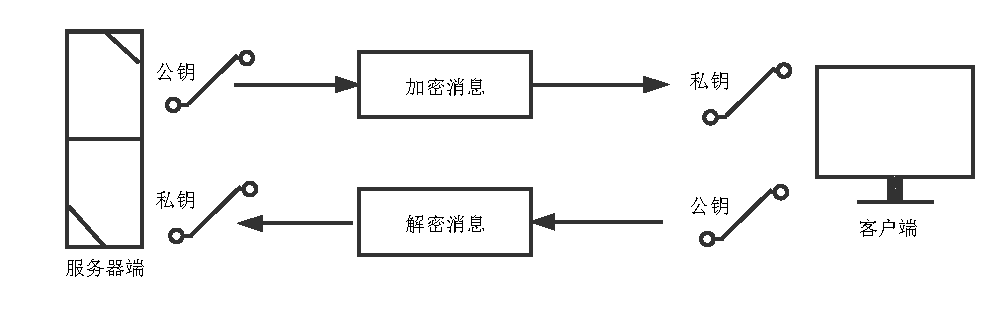
\includegraphics[scale = 0.7]{1-1.pdf}
\caption{公钥和私钥在数据传输时的角色示意图}
\end{figure}

\indent 对于 SSH 服务器和客户端来说,都基于非对称加密系统,因此SSH服务器和客户端的连接步骤如图2所示:
\begin{figure}[htbp]
\centering
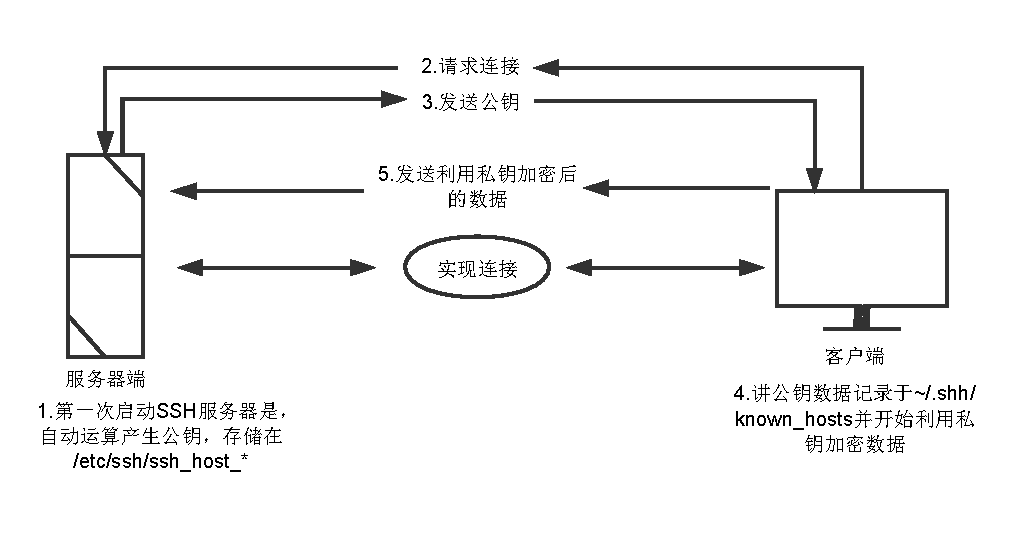
\includegraphics[scale = 0.7]{ssh.pdf}
\caption{SSH服务器与客户端的连接步骤示意图}
\end{figure}
\newpage
\section{总体概述}
采用经典的C/S 架构,将服务器端和客户端分而治之,利用Paramiko函数库快速的实现.
\subsection{安全策略}
\subsubsection{客户端安全验证}
1.(基于密码的安全验证)知道帐号和密码,就可以登录到远程主机,并且所有传输的数据都会被加密.但是,可能会有别的服务器在冒充真正的服务器,无法避免被“中间人” 攻击.\\
\indent 2.(基于
密钥的安全验证)需要依靠密钥,也就是你必须为自己创建一对密钥,并把公有密钥放在需要访问的服务器上.客户端软件会向服务器发出请求,请求用你的密钥进行安全验证.服务器收到请求之后,先在你在该服务器的用户根目录下寻找你的公有密钥,然后把它和你发送过来的公有密钥进行比较.如果两个密钥一致,服务器就用公有密钥加密“质询”(challenge)并把它发送给客户端软件.从而避免被“中间人” 攻击.
\subsubsection{服务器安全验证}
1. 在第一种方案中,主机将自己的公用密钥分发给相关的客户端,客户端在访问主机时则使用该主机的公开密钥来加密数据,主机则使用自己的私有密钥来解密数据,从而实现主机密钥认证,确保数据的保密性.\\
\indent 2. 在第二种方案中,存在一个密钥认证中心,所有提供服务的主机都将自己的公开密钥提交给认证中心,而任何作为客户端的主机则只要保存一份认证中心的公开密钥就可以了.在这种模式下,客户端必须访问认证中心然后才能访问服务器主机.

\subsection{程序流程}
对于传统的SSH 服务器和客户端设计,首先根据SSH服务器端和客户端的连接步骤设计了如下的类流程结构图,如图3所示.
\begin{figure}[htbp]
\centering
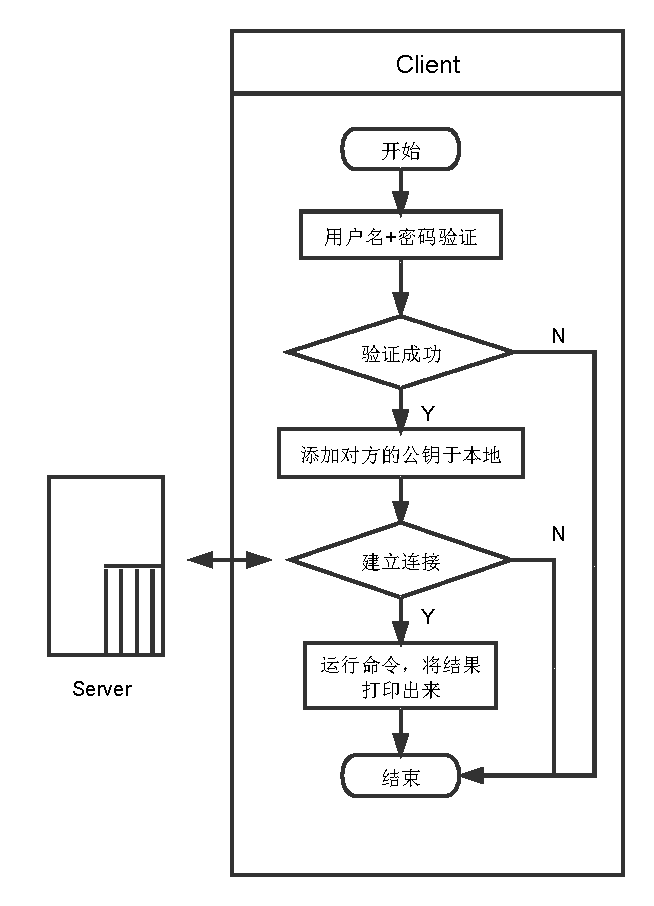
\includegraphics[scale = 0.6]{flow.pdf}
\caption{传统的SSH C/S模型结构图}
\end{figure}
\newpage
但是为了更好的设计跨平台的一个SSH服务器和客户端工具,Windows本身并不存在SSH服务器,所以经过修改传统\footnote{这里的传统指的是在UNIX或Linux平台运行的程序流程}的SSH服务器和客户端,使得在使用SSH的时候,可以反向将命令从SSH 服务器发送到客户端.

\newpage
\newpage
\section{详细设计}
\subsection{客户端设计}
在客户端实现方面,由于客户端在这里只是实现了执行对方发送过来的命令,并且将其执行的结果反向发送给对方,并在对方的显示器上反向输出出来.下面为具体实现代码.
\begin{python}
def ssh_command(ip, user, passwd, command):
	client = paramiko.SSHClient()
	# client.load_host_keys('./known_hosts')
	client.set_missing_host_key_policy(paramiko.AutoAddPolicy())
	client.connect(ip, username=user, password=passwd)
	ssh_session = client.get_transport().open_session()
	if ssh_session.active:
		ssh_session.send(command)
		print ssh_session.recv(1024)
		while 1:
			command = ssh_session.recv(1024)
			try:
				cmd_output = subprocess.check_output(command, shell=True)
				ssh_session.send(cmd_output)
			except Exception, e:
				ssh_session.send(str(e))
		client.close()
	return
\end{python}

\indent 在这里,创建了名为\textit{ssh\_command} 的函数,该函数的功能为连接到SSH 服务器并发送给服务器端一条消息,然后将服务端发送过来的消息打印出来,接着进入无限循环,在循环体内,接受服务器端发送过来的命令,然后利用\textit{subprocess.check\_output()}生成一个子进程,并且传递两个参数,在这里使用了Python的函数库:subprocess库.subprocess提供了强大的进程创建接口,在本程序中首先\textit{shell=True}表示Python将先运行一个shell,利用这个shell来解释\textit{command}命令,然后这个方法返回子进程向标准输出的输出结果,也就是说将在本机执行\textit{command}命令,并且将执行结果保存在\textit{cmd\_output}中,然后将返回结果发送给服务器端.以上为客户端执行过程.\\
\indent 另外Paramiko 支持密钥验证来代替密码验证,在现实情况下基本都为密钥认证,但是为了方便起见,在这里利用了传统的用户名和密码的方式进行验证.因为连接两端的主机(server 端和client 端)都在控制之下,所以通过设置策略\textit{paramiko.AutoAddPolicy()}自动添加和保存目标SSH 服务器的SSH 密钥.
\begin{python}
client.set_missing_host_key_policy(paramiko.AutoAddPolicy())
\end{python}

\indent \textit{set\_missing\_host\_keys}方法表示为设置连接的远程主机没有本地主机密钥或这HostKeys对象的策略,目前支持三种策略,分别为AutoAddPolicy,RejectPolicy(默认),WarningPolicy,仅限于使用于SSHClient类,其中AutoPolicy代表自动添加主机名和主机密钥到本地的HostKeys对象,并将其保存,不依赖于\textit{load\_system\_host\_keys()}的配置,即使\textit{~/.ssh/known\_hosts}不存在也不产生影响.而RejectPolicy表示自动拒绝未知未知主机名和密钥,依赖于\textit{load\_system\_host\_keys()}的配置.WarningPolicy表示用于记录一个未知的主机密钥的Python警告,并接受它,功能上与AutoAddPolicy相似,但是未知主机会有警告,但出于本项目的要求,在这里采用了AutoAddPolicy策略.\\
\indent 然后开始进行连接,最后假设连接成功,通过调用\textit{ssh\_command} 函数,发出第一条命令clientConnected
\begin{python}
ssh_command('192.168.1.3', 'administrator', 'heng130509', 'ClinetConnected')
\end{python}

\subsection{服务器端设计}
由于客户端程序较为简单,那么具体的复杂操作均在服务器端完成,首先在这里使用了Paramiko中的实例文件中的密钥,在这里主要使用了RSAKey类,接受参数,参数为密钥文件\footnote{密钥文件可以在https://raw.githubusercontent.com/paramiko/paramiko/master/tests/test\_rsa.key 下载到},这里主要的功能就是一个RSAKey可以被用于签名和验证SSH2数据.

\begin{python}
host_key = paramiko.RSAKey(filename = 'test_rsa.key')
\end{python}

\indent 开启了一个套接字监听,下面为具体实现程序:
\begin{python}
try:
	sock = socket.socket(socket.AF_INET, socket.SOCK_STREAM)
	sock.setsockopt(socket.SOL_SOCKET, socket.SO_REUSEADDR, 1)
	sock.bind((server, ssh_port))
	sock.listen(100)
	print '[+] listening for connection ...'
	client, addr = sock.accept()

except Exception, e:
	print '[-] listen failed :' +str(e)
	sys.exit(1)
\end{python}

\indent 首先利用\textit{socket.socket()}函数创建一个套接字对象,套接字构造方法的第一个参数为地址组,在这里使用了socket.AF\_INET 表示为IPv4地址族,第二个参数表示为套接字类型,在这里为TCP类型的套接字,所以在这里创建了一个TCP套接字,如果按照传统的方式做,创建完套接字对象后,然后绑定地址和端口,然后监听连接的客户端,但是在实际情况中,会出现一种情况,无论有意或者无意关闭套接字,但是还想继续始终在同一个端口上运行套接字服务器,这种情况被称作“套用套接字地址”,对于SSH服务器客户端连接来说这是非常必要的,在每次断开连接后,无需更换端口,继续保持连接,所以在这里调用了setsockopt()方法,修改地址重用状态的值,再按照常规的步骤,把套接字绑定到一个指定的地址和端口上然后启动监听,这里的最大连接数为10,然后等待连接,将一个客户端成功建立连接的时候,将接受到的客户端的套接字对象保存到client变量中,将远程建立的细节保存到addr变量中.\\
\indent 接下来会用到SSH管道,SSH管道是两台机器间的安全连接,经常被称为“SSH隧道”,或者“端口转发”。具体的实现如下:
\begin{python}
class Server(paramiko.ServerInterface):
	"""创建SSH管道"""
	def __init__(self):
		self.event = threading.Event()		
	def check_channel_request(self, kind, chanid):
		if kind == 'session':
			return paramiko.OPEN_SUCCEEDED
		return paramiko.OPEN_FAILED_ADMINISTRATIVELY_PROHIBITED
	def check_auth_password(self, username, password):
		if (username == 'administrator') and(password == 'hadoop'):
			return paramiko.AUTH_SUCCESSFUL
		return paramiko.AUTH_FAILED
\end{python}

\indent 创建一个Server类,在这里继承了paramiko.ServerInterface父类的所有属性和方法,由于paramiko.ServerInterface类调用了Paramiko主进程,所以已经基本封装了所有有关SSH服务器所有功能,在这里将不会做太多,这里创建的Server类只是在继承父类的基础上,添加一些基本的验证。首先Server类里面的\textit{\_\_init\_\_}方法时Python类的构造函数,并在类里面初始化一些变量,在这里对每个实例化类对象,都创建一个进程,\textit{check\_channel\_request}函数时继承父类的方法,然后在继承过来的方法的基础上添加了验证,\textit{check\_channel\_request}函数接受两个参数 kind 和 chanid,功能为确定一个给定类型的信道请求将被授予,并返回OPEN\_SUCCEEDED 或者错误代码。当客户端请求一个通道,验证完成后,此方法被称为服务器模式.\textit{check\_auth\_password}方法同样也是父类的方法,用来确定是否由客户提供特定的用户名和密码是用于验证身份​​接受。如果密码不被接受返回AUTH\_FAILED ,如果密码被接受则返回 AUTH\_SUCCESSFUL.\\
\indent 之后配置认证模式,代码如下:
\begin{python}
try:
	shSession = paramiko.Transport(client)
	shSession.add_server_key(host_key)
	server = Server()
	try:
			shSession.start_server(server=server)
			
	except paramiko.SSHEXceptionn, x:
		print '[-] SSH negotition failed'
\end{python}

\indent 一个SSH传输通常连接到一个网络流(通常是一个套接字),比如在这里实现的是 paramiko.Transport(client) ,就是连接了上面的接受连接的客户端的套接字对象client,然后协商加密的会话,进行身份验证,然后在整个会话中创建流隧道,称为通道. shSession.add \_server\_key(host\_key) 表示在服务器模式下添加一个主机密钥。当作为一个服务器,在SSH2协商中主机密钥用于签署某些数据包,从而使客户可以信任我们是谁。因为这是用于签名,密钥必须包含私钥信息,而不只是只有公钥。在这里传递了一个RSAKey对象的文件,然后创建Server对象,然后启动该服务。后面try...except...块为异常处理。\\
\indent 一旦服务开启之后,等待连接,当一个客户端认证成功\footnote{若连接成功,则会打印[+] Authenticaed!}  并返回 ClientConnected 消息,然后输入到\textit{sh\_sshserver} 的任何命令将发送给\textit{ sh\_sshclient} 并在 \textit{sh\_sshclient} 上执行,输出结果将返回给\textit{ sh\_sshserver}.具体实现如下
\begin{python}
while 1:
	try:
		command = raw_input("Enter command:").strip('\n')
		if command != 'exit':
			chan.send(command)
			print chan.recv(1024) + '\n'
		else:
			chan.send('exit')
			print 'exiting'
			shSession.close()
			raise Exception("Exit")
		except KeyboardInterrupt:
			shSession.close()
	except Exception, e:
		print '[-] Caught exception: ' + str(e)
		try:
			shSession.close()
		except:
			pass
		sys.exit(1)
\end{python}

\newpage

\section{测试环节}
作为示例,将在windows 主机上同时运行客户端和服务器端代码步骤如下:\\
\indent 1. 运行服务器端
\begin{figure}[htbp]
\begin{center}
  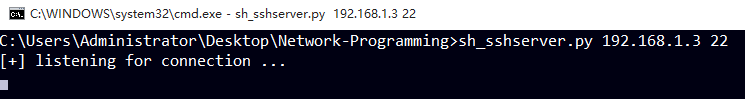
\includegraphics[width=0.8\textwidth]{1.png}
  \caption{运行服务器端}
\end{center}
\end{figure}

2. 使用客户端连接,客户端连接成功,客户端返回给服务器端ClientConnected 消息\\
\begin{figure}[htbp]
\begin{center}
  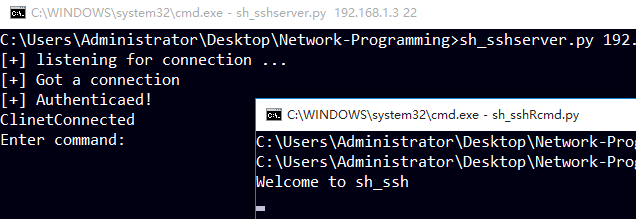
\includegraphics[width=0.8\textwidth]{2.png}
  \caption{客户端连接成功}
\end{center}
\end{figure}

3. 在服务器端执行一条命令,在客户端看不到任何情况,但是命令在客户端已经执行了,并且客户端将执行的结果返回给SSH 服务端.\\

\begin{figure}[htbp]
\begin{center}
  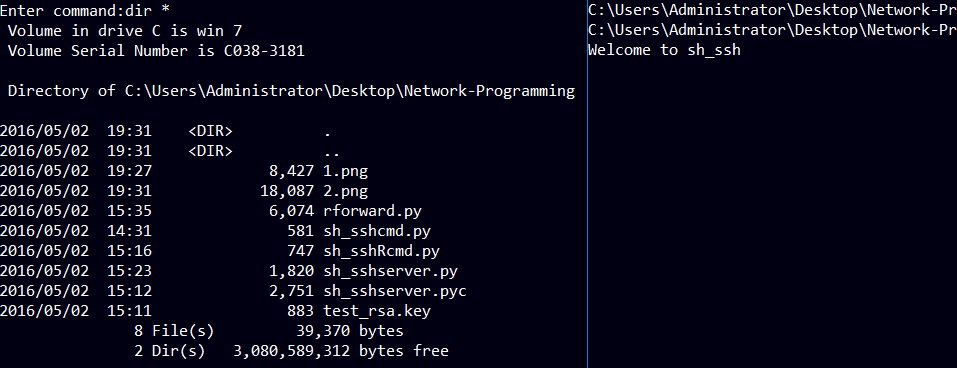
\includegraphics[width=0.8\textwidth]{3.png}
  \caption{连接成功后,在服务端执行命令,且回显打印在屏幕上}
\end{center}
\end{figure}


\newpage
\begin{thebibliography}{99}
\addcontentsline{toc}{section}{5\  \ 参考文献}

\bibitem{computer}鸟哥,鸟哥的LINUX私房菜-服务器架设篇(第三版),北京,机械工业出版社,2015,311~322
\bibitem{1}Justin Seitz,Python黑帽子-黑客与渗透测试编程之道,北京,电子工业出版社,2015,29~35
\bibitem{2}刘天斯,Python自动化运维-技术与最佳实践,北京,机械工业出版社,2015,79~103

\end{thebibliography}

\newpage
\appendix
\section{源码}

\subsection*{server.py}
\begin{python}
import paramiko
import threading
import subprocess
import sys
import socket


host_key = paramiko.RSAKey(filename = 'test_rsa.key')

class Server(paramiko.ServerInterface):
	"""docstring for Server"""
	def __init__(self):
		self.event = threading.Event()		
	def check_channel_request(self, kind, chanid):
		if kind == 'session':
			return paramiko.OPEN_SUCCEEDED
		return paramiko.OPEN_FAILED_ADMINISTRATIVELY_PROHIBITED
	def check_auth_password(self, username, password):
		if (username == 'administrator') and(password == 'hadoop'):
			return paramiko.AUTH_SUCCESSFUL
		return paramiko.AUTH_FAILED

server = sys.argv[1]
ssh_port = int(sys.argv[2])
try:
	sock = socket.socket(socket.AF_INET, socket.SOCK_STREAM)
	sock.setsockopt(socket.SOL_SOCKET, socket.SO_REUSEADDR, 1)
	sock.bind((server, ssh_port))
	sock.listen(100)
	print '[+] listening for connection ...'
	client, addr = sock.accept()

except Exception, e:
	print '[-] listen failed :' +str(e)
	sys.exit(1)

print '[+] Got a connection'

try:
	shSession = paramiko.Transport(client)
	shSession.add_server_key(host_key)
	server = Server()
	try:
		shSession.start_server(server=server)

	except paramiko.SSHEXceptionn, x:
		print '[-] SSH negotition failed'
	chan = shSession.accept(20)
	print '[+] Authenticaed!'
	print chan.recv(1024)
	chan.send('Welcome to sh_ssh')
	while 1:
		try:
			command = raw_input("Enter command:").strip('\n')
			if command != 'exit':
				chan.send(command)
				print chan.recv(1024) + '\n'
			else:
				chan.send('exit')
				print 'exiting'
				shSession.close()
				raise Exception("Exit")
		except KeyboardInterrupt:
			shSession.close()
except Exception, e:
	print '[-] Caught exception: ' +  str(e)
	try:
		shSession.close()
	except:
		pass
	sys.exit(1)
\end{python}



\subsection*{client.py}
\begin{python}
import paramiko
import threading
import subprocess

def ssh_command(ip, user, passwd, command):
	client = paramiko.SSHClient()
	# client.load_host_keys('./known_hosts')
	client.set_missing_host_key_policy(paramiko.AutoAddPolicy())
	client.connect(ip, username=user,port=8000, password=passwd)
	ssh_session = client.get_transport().open_session()

	if ssh_session.active:
		ssh_session.send(command)
		print ssh_session.recv(1024)
	while 1:
		command = ssh_session.recv(1024)
		try:
			cmd_output = subprocess.check_output(command, shell=True)
			ssh_session.send(cmd_output)
		except Exception, e:
			ssh_session.send(str(e))
	client.close()
	return
ssh_command('127.0.0.1', 'administrator', 'heng130509', 'ClinetConnected')
\end{python}

\end{document}